%%%%%%%%%%%%%%%%%%%%%%%%%%%%%%%%%%%%%%%%%
%
% (c) 2018 by Jennifer Laaser
%
% This work is licensed under the Creative Commons Attribution-NonCommercial-ShareAlike 4.0 International License. To view a copy of this license, visit http://creativecommons.org/licenses/by-nc-sa/4.0/ or send a letter to Creative Commons, PO Box 1866, Mountain View, CA 94042, USA.
%
% The current source for these materials is accessible on Github: https://github.com/jlaaser/pogil-polymers
%
%%%%%%%%%%%%%%%%%%%%%%%%%%%%%%%%%%%%%%%%%

\renewcommand{\figpath}{content/intro/M-and-D/figs}
\renewcommand{\labelbase}{M-and-D}

\begin{activity}[Molecular Weight and Dispersity]

\begin{instructornotes}

	This activity introduces students to key concepts related to the molecular weight and dispersity of polymer chains.
	
	After completing this activity, students will be able to:
			\begin{enumerate}
				\item Calculate the number-average and weight-average molecular weights of a polymer sample
				\item Calculate the dispersity of a polymer sample
				\item Interpret the dispersity of a polymer sample in terms of the standard deviation of the molecular weights
			\end{enumerate}
			
	\subsection*{Activity summary:}
	\begin{itemize}
		\item \textbf{Activity type:} Learning Cycle
		\item \textbf{Content goals:} Molecular weight and dispersity of polymer samples
		\item \textbf{Process goals:} %https://pogil.org/uploads/attachments/cj54b5yts006cklx4hh758htf-process-skills-official-pogil-list-2015-original.pdf
			written communication, critical thinking, information processing
		\item \textbf{Duration:} TBD
		\item \textbf{Instructor preparation required:} none beyond knowledge of relevant content
		\item \textbf{Related textbook chapters:}
			\begin{itemize}
				\item \emph{Polymer Chemistry} (Hiemenz \& Lodge): section 1.7
			\end{itemize}
	\end{itemize}

\end{instructornotes}

\begin{model}[Calculating Average Chain Lengths]
\label{\labelbase:mdl:MNandMW}

	Most polymer samples contain a distribution of chain lengths.  Typically, we want to know what the \emph{average} chain length is.  However, there is more than one way that we can compute an average.
	
	Consider the following set of polymer chains:
	
		\vspace{6pt}
		\centerline{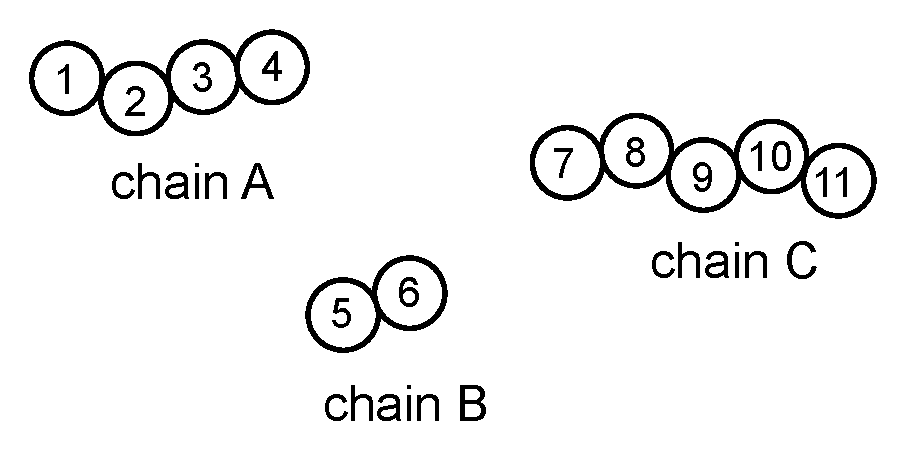
\includegraphics[width=0.65\textwidth]{\figpath/model1-polymersample}}
	
	Here, each circle denotes a single monomer.  The monomers are numbered, and each chain is assigned a letter.

\end{model}

\vspace{0.05in}
\begin{ctqs}

	\question One way we can calculate an average chain length is simply to divide the number of monomers by the number ofchains.
	
		\begin{enumerate}
		
			\item How many monomers are in the sample shown in Model \ref{\labelbase:mdl:MNandMW}?
				\label{\labelbase:ctq:nmonomers}
	
				\begin{solution}[0.5in]
					11
				\end{solution}
	
			\item How many polymer chains are in the sample shown in Model  \ref{\labelbase:mdl:MNandMW}?
				\label{\labelbase:ctq:nchains}
	
				\begin{solution}[0.5in]
					3
				\end{solution}
				
			\item Divide your answer to question \ref{\labelbase:ctq:nmonomers} by your answer to question \ref{\labelbase:ctq:nchains} to find the average chain length:
				\label{\labelbase:ctq:Mnsimple}
	
				\begin{solution}[0.75in]
					$11/3 = 3.666\dots$
				\end{solution}
				
		\end{enumerate}
	
	\clearpage
	\question A more systematic way to calculate the average from the previous problem is to average together the lengths of the chains.
				\label{\labelbase:ctq:Mncalc}
	
		\begin{enumerate}
			\item Complete the following table for the polymer samples shown in Model \ref{\labelbase:mdl:MNandMW}:
			
				\begin{center}
					\renewcommand{\arraystretch}{3}
					\begin{tabular}{|c|c|}
						\hline
						\textbf{Chain} & \textbf{Number of Monomers} \\\hline
						A     &       \answer{4}             \\\hline
						B     &       \answer{2}             \\\hline
						C     &       \answer{5}             \\\hline
					\end{tabular}
				\end{center}
				\vspace{10pt}
			
			\item Calculate the average of the numbers in the second column, and verify that it matches your result from question \ref{\labelbase:ctq:Mnsimple}:
			
				\begin{solution}[1in]
					\begin{align*}
						\frac{4+2+5}{3} = \frac{11}{3} = 3.666\dots
					\end{align*}
					
					Yes, this matches the answer from question 1c.%\ref{\labelbase:ctq:Mnsimple}.
					
				\end{solution}
			
			\item Based on your answer to the previous question, what is the average degree of polymerization of this polymer sample?
			
				\begin{solution}[0.75in]
				
					$N_{average} = 3.666\dots$
					
				\end{solution}
				
			\item If each monomer has a molecular weight of 100~g/mol, what is the average molecular weight of the chains?
			
				\begin{solution}[1in]
				
					$M_{average} = N_{average}M_0 = (3.666\dots)(100\text{ g/mol}) = 366.666\dots\text{ g/mol}$
				
				\end{solution}
				
		\end{enumerate}
	
	\clearpage
	\question Another way we can calculate an average chain length is to count each chain once for each monomer it contains.
				\label{\labelbase:ctq:Mwcalc}
	
		\begin{enumerate}
			\item Fill in the missing entries in the following table:
			
				\begin{center}
					\renewcommand{\arraystretch}{2.25}
					\begin{tabular}{|c|c|c|}
						\hline
						\textbf{Monomer number...} & \textbf{is in chain...} & \textbf{which contains this many monomers:} \\ \hline
						1                   & A                       & 4                                           \\ \hline
						2                   & A                       &                                           4 \\ \hline
						3                   & A                        &                                            4 \\ \hline
						4                   & A                        &                                            \answer{4} \\ \hline
						5                   & B                        &                                            \answer{2} \\ \hline
						6                   & B                        &                                            \answer{2} \\ \hline
						7                   & C                        &                                            \answer{5} \\ \hline
						8                   &  \answer{C}                      &                                             5 \\ \hline
						9                   & \answer{C}                        &                                            5 \\ \hline
						10                  &  \answer{C}                       &                                            5 \\ \hline
						11                  &  \answer{C}                       &                                            5 \\ \hline
					\end{tabular}
				\end{center}
			
			\item Calculate the average of the numbers in the third column:
			
				\begin{solution}[1.5in]
				
					\begin{align*}
						\frac{4+4+4+4+2+2+5+5+5+5+5}{11} = \frac{45}{11} = 4.09
					\end{align*}
				
				\end{solution}
			
			\item Based on your answer to the previous question, what is the average degree of polymerization of this polymer sample?
			
				\begin{solution}[0.75in]
					4.09
				\end{solution}
				
			\item If each monomer has a molecular weight of 100~g/mol, what is the average molecular weight of the chains?
			
				\begin{solution}[0.75in]
					(4.09)(100 g/mol) = 409 g/mol
				\end{solution}
				
		\end{enumerate}
		
	\question Do the approaches in questions \ref{\labelbase:ctq:Mncalc} and \ref{\labelbase:ctq:Mwcalc} give you the same average molecular weight?  If not, why not?  Explain your reasoning in 2-3 complete sentences.
	
		\begin{solution}[3in]
			No, the answers do not agree.  The approach in question \ref{\labelbase:ctq:M2calc} gave a larger number than the approach in question 2. %\ref{\labelbase:ctq:Mncalc}.  
			This is because the second approach counts each chain multiple times, so larger chains contribute more to the average.
		\end{solution}
		
\end{ctqs}

\begin{infobox}
	
	The two main types of averages that we use in polymer science are the \emph{number-average} and \emph{weight-average} molecular weights.
	
	The number-average molecular weight is given by
	\begin{equation*}
		M_n = M_0 \frac{\sum_i i \cdot n_i}{\sum_i n_i}
	\end{equation*}
	while the weight-average molecular weight is given by
	\begin{equation*}
		M_w = M_0 \frac{\sum_i i^2 \cdot n_i}{\sum_i i\cdot n_i}
	\end{equation*}
	
	In both of these expressions, $n_i$ is the number of chains with $i$ monomers and $M_0$ is the molecular weight of a single monomer.
	
\end{infobox}


\begin{ctqs}

	\question Fill in the missing entries in the following table for the polymer sample shown in Model \ref{\labelbase:mdl:MNandMW}:
			
				\begin{center}
					\renewcommand{\arraystretch}{3}
					\begin{tabular}{|c|c|c|c|}
						\hline
						\textbf{$i$} & \textbf{$n_i$} & \textbf{$i\cdot n_i$} & \textbf{$i^2\cdot n_i$} \\\hline
						1 & 0 & 0 & 0 \\\hline
						2 & 1 & 2 & 4 \\\hline
						3 & 0 & \answer{0} & \answer{0} \\\hline
						4 & 1 & 4 & \answer{16} \\\hline
						5 & \answer{1} & \answer{5} & \answer{25} \\\hline
						\textbf{Sum of column values:} & $\sum_i n_i=3$ & $\sum_i i\cdot n_i =$\hspace{0.5cm}\answer{11}\hspace{0.5cm} & $\sum_i i^2 \cdot n_i = $\hspace{0.5cm}\answer{31}\hspace{0.5cm} \\\hline
					\end{tabular}
				\end{center}
	
	\question Using the values in the last row of this table, and the provided equations, calculate $M_n$ and $M_w$ for the polymer sample shown in Model \ref{\labelbase:mdl:MNandMW}.  Remember that the molecular weight of each monomer is 100~g/mol.
	
		\begin{solution}[1.5in]
		\end{solution}
	
	\question In questions \ref{\labelbase:ctq:Mncalc} and \ref{\labelbase:ctq:Mwcalc}, which approach gave the number-average molecular weight, and which gave the weight-average molecular weight?
	
		\begin{solution}[1.5in]
		\end{solution}
	
	\question For the polymer sample shown in Model \ref{\labelbase:mdl:MNandMW}, $M_w$ was larger than $M_n$.  Is this always true, or are there cases where $M_w$ could be smaller than $M_n$?  Briefly defend your answer in 1-2 complete sentences.
	
		\label{\labelbase:ctq:MWvsMN}
		
		\begin{solution}[2in]
		
			It is always true that $M_w \geq M_n$.  This is because the calculation for $M_w$ ``counts'' the larger/heavier chains more times than the smaller/lighter chains, making the average value larger than for $M_n$ (in which all chains are counted the same number of times).
			
		\end{solution}
	
	%\question OFTEN WANT TO CONVERT BETWEEN MW and DP - EQNS TO CONVERT? 
		
\end{ctqs}

\begin{model}[Distributions of Chain Lengths]
\label{\labelbase:mdl:dispersity}

	Several different polymer samples are shown below:
	
	\vspace{6pt}
	\centerline{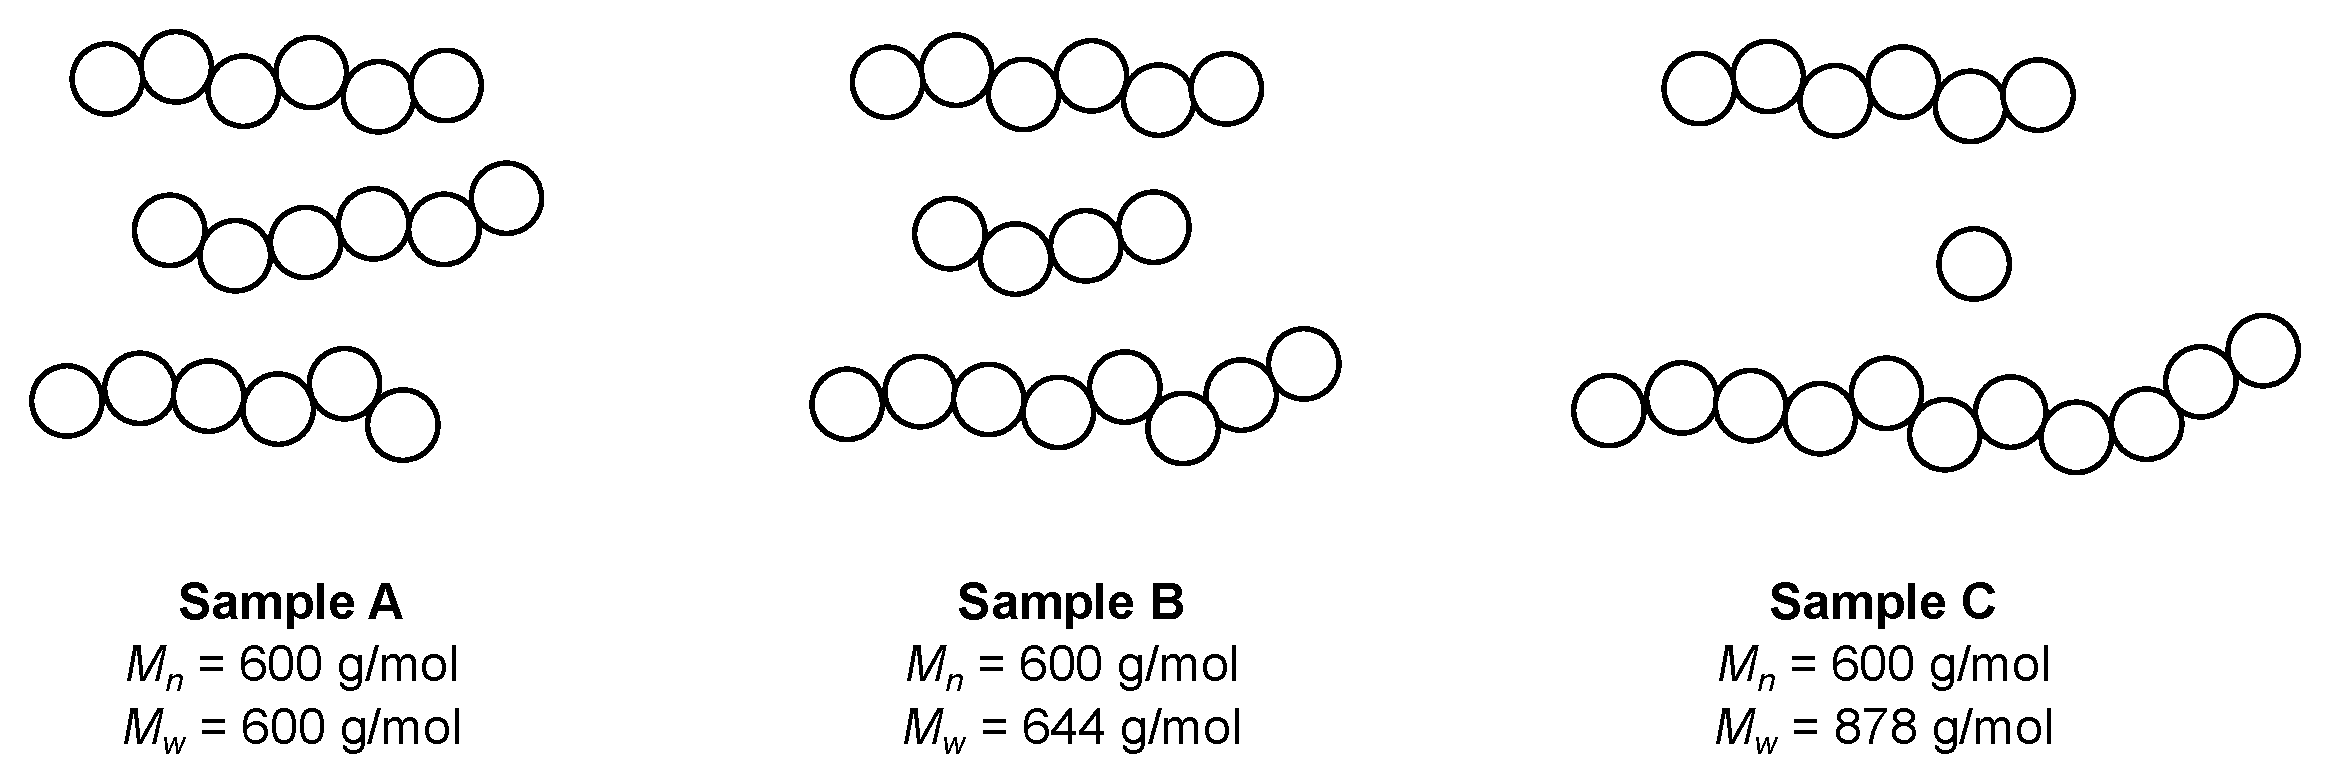
\includegraphics[width=0.9\textwidth]{\figpath/model2-samples}}

\end{model}
	
\begin{ctqs}

	\question Briefly describe your qualitative observations about how $M_n$ and $M_w$ change with distribution of chain lengths in the samples shown in Model \ref{\labelbase:mdl:dispersity}:
	
		\begin{solution}[2in]
		\end{solution}
	
\end{ctqs}

\begin{infobox}

	The relationship between $M_n$ and $M_w$ can be summarized by a quantity called the \emph{dispersity}.  The dispersity of a polymer sample, denoted, \PDItext, is defined as
	\begin{equation*}
		\PDImath = \frac{M_w}{M_n}
	\end{equation*}
	
\end{infobox}

\begin{ctqs}

	\question Calculate the dispersity of each of the polymer samples shown in Model \ref{\labelbase:mdl:dispersity}.
	
				\begin{center}
					\renewcommand{\arraystretch}{4}
					\begin{tabular}{|c|c|}
						\hline
						\textbf{Sample} & \hspace{2cm}\textbf{\PDItext}\hspace{2cm} \\\hline
						A     &       \answer{1}             \\\hline
						B     &       \answer{1.07}             \\\hline
						C     &       \answer{1.46}             \\\hline
					\end{tabular}
				\end{center}
				\vspace{10pt}
	
	\question Describe, in your own words, what it means when the dispersity is...
	
		\begin{enumerate}
			\item ... equal to 1:
			
				\begin{solution}[0.75in]
				\end{solution}
			
			\item ... slightly greater than 1:
			
				\begin{solution}[0.75in]
				\end{solution}
			
			\item ... much greater than 1:
			
				\begin{solution}[0.75in]
				\end{solution}
			
		\end{enumerate}
		
	\question Can the dispersity ever be less than one?  Briefly justify your answer in 1-2 complete sentences.
	
		\begin{solution}[2in]
			No. Because the weight-average molecular weight is always greater than the number-average molecular weight (see question 8, %\ref{\labelbase:ctq:MWvsMN}), 
			the dispersity will always be greater than or equal to one.
		\end{solution}
	
\end{ctqs}



\begin{exercises}

		\exercise The equations for $M_n$ and $M_w$ given in the activity are given in terms of $n_i$, the number of chains with degree of polymerization $i$, and $M_0$, the molecular weight of a single monomer.
		
		Show that each of the following are equivalent expressions for $M_n$ and $M_w$:
		
			\begin{enumerate}
				
				\item \begin{align*}
					M_n = \frac{\sum_i n_i M_i}{\sum_i n_i} && \text{and} &&  M_w = \frac{\sum_i n_i M_i^2}{\sum_i n_i M_i}
				\end{align*}
					where $n_i$ is the number of chains of length $i$ and $M_i$ is the molecular weight of each chain of length $i$.
				
				\item  \begin{align*}
					M_n = \sum_i x_i M_i && \text{and} && M_w = \sum_i w_i M_i
				\end{align*}
					where $x_i$ is the \emph{mole fraction} of chains that have length $i$, and $w_i$ is the \emph{weight fraction} (fraction of the total mass) that comes from chains of length $i$.
				
			\end{enumerate}
			
		\exercise Calculate the number-average and weight-average molecular weights of...
		
			\begin{enumerate}
			
				\item ... a sample that contains 1 mole each of hexane (\ce{C6H14}) and undecane (\ce{C12H26}).
				
				\item ... a sample that contains 1 gram each of hexane (\ce{C6H14}) and undecane (\ce{C12H26}).
				
			\end{enumerate}
			
		\exercise The standard deviation in the molecular weights of a sample are related to the dispersity by
		
			\begin{align*}
					\sigma = M_n\sqrt{\PDImath - 1}
			\end{align*}
			
			\begin{enumerate}
				\item What is the standard deviation in the molecular weight for a sample with $M_n=25$~kg/mol and $\PDImath=1.25$?
				
				\item How small would the dispersity need to be for the standard deviation to be less than 10\% of $M_n$?
			\end{enumerate}
			
\end{exercises}
	
\end{activity}